%focus on sub-goal
\chapter{Design and Implementation}\label{chapter:prototype_implementation}

Implementing an evolutionary algorithm requires a number of considerations. A robust fitness assignment method needs to be determined. A mechanism for uniform diversity preservation must be conceptualized. Also, a well-thought-out solution to handle constraints from the problem definition must be designed. Luckily, there are successful evolutionary algorithms that can be used in practice. Such algorithms have been well researched, and their domain applicability is well-defined. 

\Gls{nsga}-II \parencite{Jain2013AnOptimization} is an evolutionary algorithm that uses an elitist non-dominated sorting mechanism. It is an improved version of an initial \gls{nsga} algorithm, developed by  Srinivas et al. \parencite{Srinivas1994MuiltiobjectiveAlgorithms} in 1996. 
\Gls{nsga}-II uses concept like crowding function for diversity preservation and ranking of the Pareto fronts. However, it is better suited for bi-objective problems and does not perform well for multiple objective problems. \Gls{nsga}-III \parencite{Mkaouer2015Many-objectiveNSGA-III} was introduced to solve the inability of \gls{nsga}-II to solve many objective problems (i.e., three or more objectives).

Other successful evolutionary algorithms that are applicable to our problem can also be found in practice. In the following sections, we shall be adapting the \gls{nsga} algorithm and its variants to our problem definition.

\section{Non-Dominated Sorting Genetic Algorithms}
Designing domination based \gls{emo} algorithms for many objective problems requires additional considerations. For one, an increase in the number of objectives may cause an increase in non-dominated population from the population of randomly generated population. Since domination based \gls{emo} prioritizes non-dominated solutions, the solution space becomes rather large. Hereby, the search process becomes slow, and the algorithm becomes inefficient. Also, with the increased solution space arises an increase in the number of neighbors. Evaluation of diversity measures (i.e., crowding distance) becomes computationally expensive. \gls{nsga}-III was designed to address these problems. 

As defined in \ref{sec:problem_definition}, our problem can be mapped to a many objective optimization problem. Each objective function is a function of a \gls{poi} and its characteristics. A chosen algorithm needs to be able to efficiently compare more than three objectives. Thus, this informs the decision to implement and adapt the \gls{nsga}-III to our problem domain. Going forward, we shall be exploring the intrinsic parts that comprises the \gls{nsga}-III and will constitute our algorithm.



\subsection{The NSGA-III Algorithm}
The \gls{nsga}-III algorithm was developed to address the inefficiency of \gls{nsga}-II for handling many objective problems. In its most basic form, it can be seen as the \gls{nsga}-II algorithm with minor changes. That is, most algorithmic step in \gls{nsga}-III are from the \gls{nsga}-II algorithm. Figure \ref{fig:nsgaII} and \ref{fig:nsgaIII} respectively depict an overview of the major algorithmic steps of the \gls{nsga}-II and \gls{nsga}-III. From these figures, one can observe the similarity between both algorithms. However, a major difference between both algorithms is the last step of the next population generation. Unlike \gls{nsga}-II that uses crowding distance sorting of individuals to decide what part of a Pareto front to reject or accept, \gls{nsga}-III uses a reference point based sorting technique. The crowding distance sorting technique has been explained in section \ref{sec:diversitypreservation}. Reference point based sorting technique and other intrinsic details of the \gls{nsga}-III shall be explained subsequently.

\begin{figure}
    \centering
    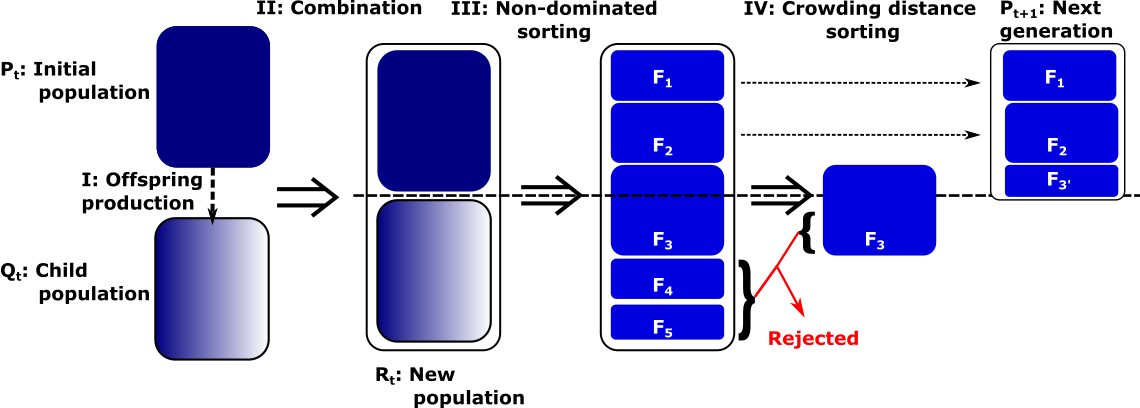
\includegraphics[width=9cm]{NSGA-II}
    \caption{NSGA-II Overview}
    \label{fig:nsgaII}
\end{figure}

\begin{figure}
    \centering
    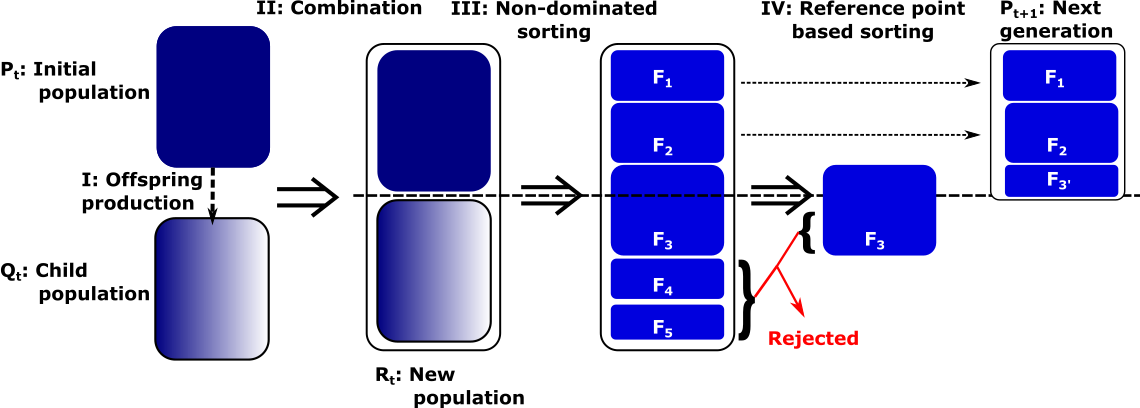
\includegraphics[width=9cm]{NSGA-III}
    \caption{NSGA-III Overview}
    \label{fig:nsgaIII}
\end{figure}

\subsubsection{Initial Population}
Let us consider $P_t$ as a parent population of the $t-th$ generation of the algorithm (i.e., iteration $t$). $P_t$ with $N$ chromosomes, is either a population gotten from previous generation $t-1$ or an initial population gotten from a defined heuristic.\\ 
The heuristic used for initial population generation at the start of the algorithm is particularly important for our problem. Just randomly sampling from the problem space will be logically inefficient. Many objective problems in practice are typically capped at 15-20 objective problems. \Gls{nsga}-III was evaluated on 20-Objective DTLZ1-DTLZ2. Considering that the objective function in our problem domain comprises a single \gls{poi} and its characteristics, an intelligent preselection process has to be defined, to reduce the problem space.

\subsubsection{Constraint Handling}
Figure \ref{fig:unconstrainedsearchspace} illustrates a typical solution search space of an unconstrained problem. For unconstrained problems, all members of the population are regarded as feasible. However, in unconstrained problems (figure \ref{fig:constrainedserachspace}), some individuals become infeasible (i.e., members in gray shaded area). Additional techniques are needed for handling constraints in \gls{nsga}-III. Two different papers were published for \gls{nsga}-III on problems without constraints \parencite{Deb2013AnConstraints} and on problems with constraints \parencite{Jain2013AnApproach}. 

\begin{figure}[h!]
\centering
\subfloat[Unconstrained Solution Search Space]{
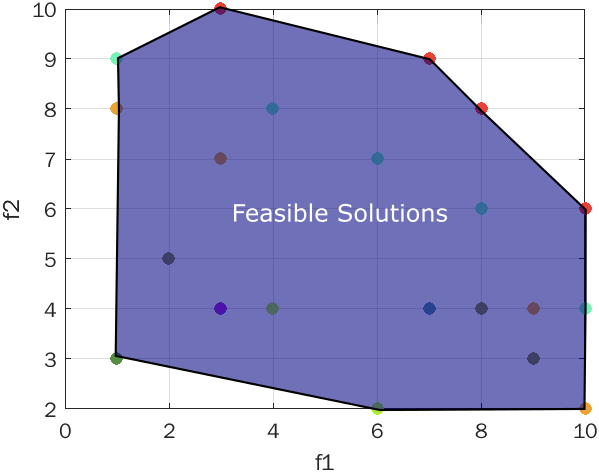
\includegraphics[width=.4\textwidth]{UnconstrainedSolutionSpace}
\label{fig:unconstrainedsearchspace}}\qquad
\subfloat[Constrained Solution Search Space]{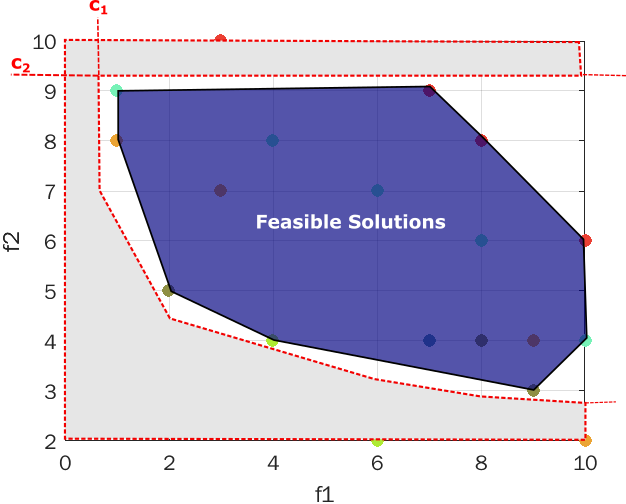
\includegraphics[width=.4\textwidth]{ConstrainedSearchSpace}
\label{fig:constrainedserachspace}}
\caption{Solution Search Space}
\label{fig:constrainedvsunconstrained}
\end{figure}

Let us consider an individual $x$ in the solution space and the following constraints:
\begin{align}
    \tag{constraint 1 }g_j(x) \leq b_j \label{eq:4a}\\
    \tag{constraint 2}h_k(x) = 0 \label{eq:4b}
\end{align}
The paper \parencite{Jain2013AnApproach} suggests calculating a constraint valuation value $CV(x)$ to measure the degree to which $x$ violates the constraints using the following formula:
\begin{align*}
    CV(x) = \sum_{j=1}^J \langle g'_j(x)\rangle + \sum_{k=1}^K \lvert h'_k(x)\rvert
\end{align*}
where $g'_j(x)$ is the normalized constraint function for constraint \ref{eq:4a}, such that $g'_j(x) = g_j(x) / b_j  - 1 \leq 0$ and $h'_k(x)$ is the normalized constraint function for constraint \ref{eq:4b}. The angle bracket operator $\langle \alpha \rangle$ returns the negative of $\alpha$, if $\alpha < 0$ and returns zero, otherwise. Assuming constraint \ref{eq:4a} was a greater or equals constraint (i.e., $g_j(x) \geq b_j$), then $\langle \alpha \rangle$ returns the negative of $\alpha$, if $\alpha > 0$ and returns zero, otherwise.

The notion of feasibility, together with the constraint violation measure $CV(x)$, are combined to derive a \textit{constraint dominates} principle. 
Let us once more consider two individuals $x_1$ and $x_2$ in the solution space. An individual $x_1$ is said to constraint dominate $x_2$ if any of the following conditions holds:
\begin{enumerate}
    \item $x_1$ is feasible and $x_2$ is infeasible;
    \item Both $x_1$ and $x_2$ are infeasible and $x_1$ has a lower \gls{cv} value;
    \item Both $x_1$ and $x_2$ are feasible and $x_1$ dominates $x_2$ ($x_1 \succ x_2$).
\end{enumerate}




\subsubsection{Offspring Production}
Three major aspects for generating the child population $Q_t$ are defined as follows:

\begin{enumerate}
    \item \textbf{Tournament Selection}: To selection two individuals that will be eligible to produce offspring for the next generation, a tournament selection procedure occurs. Two individuals are selected from $P_t$ at random and a binary selection of the better solution is applied as shown in algorithm \ref{alg:tournament_selection}. Individuals $p_1$ and$p_2$ are compared to each other to select one that does not violate the constraints. If both individuals violate the constraints, the constraint violation value for both individuals is computed. Then, the algorithm selects the individual with the lesser constraint violation value. Two parents for reproduction (cross over and mutation) are selected using this tournament procedure.
    \item \textbf{Cross over}: A crossover operator is used to generate offsprings according to a crossover rate $p_c$. The crossover rate represents the proportion of parents on which a crossover operator will act. A uniform crossover will ensure that each offspring will inherit some characteristics of both parents. However, the 1-point crossover or the n-point crossover is commonly used for binary representations. In the 1-point crossover, a crossover site $k$ is randomly selected. Then two offsprings are created by exchanging the segments of the parents \parencite{Talbi2009Metaheuristics:Implementation}. Consequently, n-point crossover implies $n$ crossover sites. 
    %The most commonly used rates are in the interval [0.45, 0.95]. Adaptive techniques for the crossover rate may also be useful
    \item \textbf{Mutation}: Mutation operators act on a single individual. An element of the representation is mutated (changed) according to some probability $p_m$. \parencite{Talbi2009Metaheuristics:Implementation} recommends small values for $p_m$ ($p_m \in [0.001, 0.01]$). The flip operator is commonly used when using binary representation of individuals. %Some strategies initialize the mutation probability to 1/k where k is the number of decision variables, that is, in average only one variable is mutated.
    
\end{enumerate}
During reproduction, duplicate offsprings are checked and eliminated. A child population $Q_t$ of size $N$ is generated by repeating tournament selection and reproduction. $R_t$ is generated by combining $P_t$ and $Q_t$ (i.e., $R_t = P_t \cup Q_t$). \Gls{nsga}-III (and also \gls{nsga}-II) use an elitist preservation technique (III and IV from figure \ref{fig:nsgaIII}) to preserve elite members of the new population. 

\begin{algorithm}[h!]
  \caption{Tournament Selection Procedure}\label{alg:tournament_selection}
  \SetKwInOut{Input}{Input}
  \SetKwInOut{Output}{Output}
  \Input{$p_1$, $p_2$}
  \Output{$p'$}
    \uIf{feasible($p_1$) and not feasible($p_2$)}
    {
        $p' = p_1$
    }
    \ElseIf{not feasible($p_1$) and feasible($p_2$)}
    {
        $p' = p_2$
    }
    \ElseIf{not feasible($p_1$) and not feasible($p_2$)}
    {
        \If{CV($p_1$)  $>$ CV($p_2$)}
        {
            $p' = p_2$
        }
        \ElseIf{CV($p_1$)  $<$ CV($p_2$)}
        {
            $p' = p_1$
        }
        \Else{
            $p' = random(p_1, p_2)$
        }
    }
    \ElseIf{feasible($p_1$) and feasbile($p_2$)}
    {
        $p' = random(p_1, p_2)$
    }
    
  \end{algorithm}

\subsubsection{Non-dominated Sorting}
Non-dominated sorting ranks members of the population $R_t$ into different non-dominated levels ($F_1$, $F_2$, and so on) according to their constraint domination count. We introduce a new symbol $\succ_+$ for constraint domination. For example, let $A$, $B$, and $C$ be selected members of the population  such that $A \succ_+ B \succ_+ C$ (i.e., $A$ constraint dominates $B$ and $C$, $B$ constraint dominates $C$). Figure \ref{fig:paretolevels} depicts $A$, $B$, and $C$ on a graph. $A$ will have the highest domination count and hence belong to domination level $F_1$. $B$ will belong to $F_2$ and $C$ to $F_2$. 

\begin{figure}
\centering
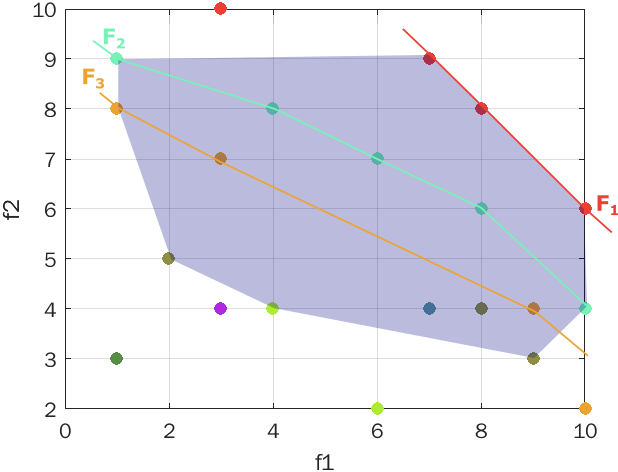
\includegraphics[width=.5\textwidth]{NonDominatedFronts}
\caption{Ranking of Pareto Frontier according to Constrained Domination}\label{fig:paretolevels}
\end{figure}

Thereafter, the number of feasible solutions $N_f$ in $R_t$ are counted. If $N_f \leq N$, all the feasible solutions are added to $S_t$ for starting the next generation $P_{t+1}$. The remaining $K = N - \lvert P_{t+1} \rvert$ population slots are filled with top level infeasible solutions, that is, solutions having smaller \gls{cv} values.\\
If $N_f > N$, the algorithm follows the unconstrained selection procedure described in \parencite{Deb2013AnConstraints}. Each level is selected one at a time until a size $N$ is reached or $N$ is for the first time exceeded. Assuming the $lth$ level is the level that causes the size of $S_t$ to exceed $N$, then solutions in the level $l$ will only partially be accepted into $S_t$. 
%niche-preservation operator that computes the crowding distance for every last level member as the summation of objective-wise normalized distance between two neighboring solutions. 

\subsubsection{Reference Point Based Sorting}
\Gls{nsga}-III uses a predefined set of reference points to ensure diversity in solutions. The reference points can either be preferential points supplied by the user or predefined in a structure manner \parencite{Deb2013AnConstraints}. \\ 
In the case of structured reference points, it uses a systematic approach that creates points on a normalized hyperplane. Different points are placed on a
normalized hyperplane that have the same orientation in
all axis. The total number of reference points ($H$) is given by:
\begin{align*}
    H &= \begin{pmatrix}
    M + p - 1 \\
    p
    \end{pmatrix}
\end{align*}
where $M$ is the number of objective functions and $p$ is the number of divisions to consider along each objective. For example, using three objectives ($M = 3$) and four divisions ($p = 4$), the reference points are placed on a triangle with its apex at $(1,0,0), (0,1,0),$ and $(0,0,1)$. $H = \big(\begin{smallmatrix}
  6\\
  4
\end{smallmatrix}\big)$, thus 15 reference points will be created. The obtained reference points are widely distributed on the entire normalized hyperplane, and the solutions are also widely distributed on or near the Pareto-optimal front. Population members that are associated with the created reference points are emphasized. The population size is recommended to be the smallest multiple of four, greater than $H$. In the case of user-supplied reference points, the user can mark $H$ points on the normalized hyperplane.

After determining the reference points on a hyperplane, the algorithm \textit{adaptively normalizes the population members}. First, the ideal point\footnote{The algorithm presented in the paper focused on minimization problems, thus the ideal point was differently defined. Since, we are faced with a maximization problem, our ideal point is defined differently.} of the population $S_t$ is determined by identifying the maximum value ($z_i^{max}$) for each objective function $i = 1, 2,...., M$ in $\cup_{\tau=0}^{t} S_\tau$ and by constructing the ideal point $\Tilde{z} = (z_1^{max}, z_2^{max},..., z_M^{max})$. Using $f'_i(x) = z_i^{max} - f_i(x)$, each objective value of $S_t$ is translated. Thereafter, the extreme point ($z_i^{ext}$) in each objective axis is identified. Given  a weight vector $d_i$, which is close to the ith objective axis, an achievement scalarizing function (ASF) is given by:
\begin{align*}
    ASF(x, d_i) = max_{k=1}^M \frac{f'_i(x)}{d_i}, \qquad for\ i = 1, 2,...,M. 
\end{align*}
$z_i^{ext}$ is identified by finding a solution ($x \in S_t$) that makes the corresponding ASF minimum. These $M$ extreme vectors are then used to represent a $M$ dimensional hyperplane. The intercept $a_i$ of the ith objective axis and the linear axis can then be calculated by $a_i = z_i^{max} - z_i^{ext}$. These maximum and extreme values are
updated at every generation using the current population. Putting it all together, the objective function can be normalized by:
\begin{align}
    f_i^n(x) &=  \frac{z_i^{max} - f_i(x)}{z_i^{max} - z_i^{ext}}, \qquad for\ i = 1, 2,...,M. \label{eq:41a}  
\end{align}

After normalizing the objective functions, each population member is \textit{associated with a reference point}. A reference line for each reference point on the hyperplane is defined by joining the reference point with the ideal point. Then a perpendicular distance among each population member and each reference line is calculated. The reference point that has the closest reference line to a population individual in the normalized objective space is considered to be associated with the population individual.

A \textit{niche-preserving procedure} to generate the remaining $K = N - \lvert P_{t+1} \rvert $ population slots is performed. A reference point may have one or more population members associated with it. It might also not have any associated reference point. Initially, the number of population members from $P_{t+1} = S_t \setminus F_l$ that are associated with the jth reference point are counted each as $\rho_j$ (niche count). Then, the reference point set $J_{min} = {j:argmin_j \ \rho_j}$ having minimum $\rho_j$ is identified. In case of multiple such reference points, a random $\Tilde{j} \in J_{min}$ is selected from $J_{min}$. 
If there is no associated $P_{t+1 }$ member to the reference point $\Tilde{j}$ ($\rho_{\Tilde{j}} = 0$), then either of the following scenario is possible: 
\begin{enumerate}
    \item There exists one or members in front $F_l$ that are associated with the reference point $\Tilde{j}$; or
    \item The front $F_l$ does not have any member associated with the reference point $\Tilde{j}$.
\end{enumerate}
In case 1, the reference point the shortest perpendicular distance from the reference line is added to $P_{t+1}$, then the count $\rho_{\Tilde{j}}$ for the reference point $\Tilde{j}$ is incremented by one. In case 2, the reference point is excluded from further consideration for the current generation.\\
In the event that $\rho_{\Tilde{j}} \geq 1$, a randomly chosen member, if exists, from the front $F_l$ that is associated with the reference point $\Tilde{j}$ is added to $P_{t+1}$. $\rho_{\Tilde{j}}$ is the incremented by one. The procedure is repeated $K$ times until all vacant slots in $\rho_{\Tilde{j}}$ are filled.



\section{Algorithmic Approaches}
In this section, several approaches to solve the many-objective orienteering problem present in \ref{sec:problem_definition} are presented. An approach describes an optimization process that comprises varying \textit{initialization} steps, and \textit{constraint handling techniques}.

\subsection{Start Population}
The first step in each approach is to initialize the first population from which the evolutionary algorithm begins. The performance of the algorithm can vary depending on the starting population used. A main criterion is a good diversity at the beginning of the optimization process. Three different initialization techniques are chosen and described below. The first initialization method is a naive method that randomly samples a part of the population. We adapt the metric used in \parencite{cbrecsys2014} to create a second method which generates feasible solutions only. The third method works similar to the second method, but relaxes the similarity metric used.

\subsubsection{Random Initialization}

\subsubsection{Rate-Based Initialization I}

\subsubsection{Rate-Based Initialization II}


\subsection{Constraint Handling Technique}

\subsubsection{p-Dominates}
\subsubsection{constraint dominates}
\subsubsection{hybrid}
\subsubsection{adaptive penalty}
hybrid (penalty based, non-penalty based, mixed)
\subsubsection{Adaptive Normalization}
p-dominates for penalty based full, and mixed
\section{General Framework}

\subsection{Stopping Criteria}




